%  !TeX  root  =  user_guide.tex

\section{Модуль захвата координат}\label{coordcapt}

% когда переработка раздела будет завершена,
% раскоментируйте следующую строку:
% \updatedisclaimer

Модуль захвата координат прост в использовании и обеспечивает возможность
отображать координаты на поле карты в двух определённых системах координат.

\begin{figure}[ht]
   \centering
   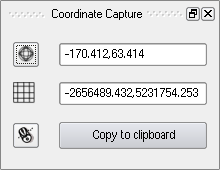
\includegraphics[clip=true, width=8cm]{coordinate_capture_dialog}
   \caption{Модуль захвата координат \wincaption}\label{fig:coordinate_capture_dialog}
\end{figure}

\begin{enumerate}
  \item Запустив QGIS, выберите \dropmenuopttwo{mActionOptions}{Свойства проекта} в меню
  \mainmenuopt{Установки} (KDE, Windows) или \mainmenuopt{Файл} (Gnome, OS\,X)
  и выберите вкладку \tab{Система координат}. Также вы можете открыть данный модуль,
  используя кнопку \toolbtntwo{mIconProjectionEnabled}{Преобразование координат}
  в нижнем правом углу окна программы на панели статуса.
  \item Отметьте пункт \checkbox{Включить преобразование координат «на лету»}
  и выберите нужную систему координат проекта (см. также Раздел~\ref{label_projections}).
  \item Загрузите модуль захвата координат в Менеджере модулей (см. Раздел~\ref{sec:load_core_plugin})
  и убедитесь что в меню \mainmenuopt{Вид} \arrow \dropmenuopt{Панели}
  отмечен пункт \checkbox{Захват координат}.
  Диалоговое окно модуля захвата координат представлено на
  рисунке~\ref{fig:coordinate_capture_dialog}.
  \item Щелкните по кнопке \toolbtntwo{geographic}{Щелкните для выбора
  системы координат, используемой для вывода} и выберите в диалоговом окне
  требуемую систему координат.
  \item Для запуска захвата координат щелкните по кнопке \button{Начать захват}.
  Теперь вы можете щелкнуть в любом месте поля карты, и в модуле отобразятся
  координаты выбранного места в требуемой системе координат.
  \item Кнопка \toolbtntwo{tracking}{слежение за курсором} позволяет включить
  режим слежения за курсором мыши.
  \item Также имеется возможность скопировать выбранные координаты в буфер обмена.
\end{enumerate}

\FloatBarrier
